\documentclass{beamer}
\usepackage{listings}
\usepackage{graphicx}
\usepackage{hyperref}
\usepackage{array}

\setlength{\tabcolsep}{1pt}

\usetheme{Madrid}

\title{Trie Benchmark Evaluation}
\author{Robert Andreas Fritsch}
\date{\today}

\begin{document}

% Title slide
    \begin{frame}
        \titlepage
        Vorlesung: Text-Indexierung WiSe 24/25\\
    \end{frame}

% Evaluation Slide (fragile because of verbatim content)
    \begin{frame}[fragile]{Evaluation}
        All benchmarks are run on:
        \begin{verbatim}
Intel(R) Core(TM) i5-8250U CPU @ 1.60GHz
RAM  (DDR4):           7.6Gi
Swap (NVMe PCIe SSD): 63.0Gi
        \end{verbatim}

        \vspace{0.5cm}
        Run command:
        \begin{verbatim}
taskset -c $CORE sudo chrt -f 99 ./benchmark
        \end{verbatim}
    \end{frame}

% --- Variation Slides ---

    \begin{frame}[fragile]{Variation: Vector Trie}
        \begin{lstlisting}[basicstyle=\ttfamily\small, frame=single]
struct Node
{
  bool is_end = false;
  std::vector<std::pair<unsigned char,
                        std::unique_ptr<Node>>> children;
};
        \end{lstlisting}
    \end{frame}

    \begin{frame}[fragile]{Variation: Array Trie}
        \begin{lstlisting}[basicstyle=\ttfamily\small, frame=single]
struct Node
{
  std::size_t is_end = false;
  std::unique_ptr<Node> children[63];
  Node() { static_assert(sizeof(Node) == 64 * 8); }
};
        \end{lstlisting}
    \end{frame}

    \begin{frame}[fragile]{Variation: Hash Trie}
        \begin{lstlisting}[basicstyle=\ttfamily\small, frame=single]
struct Node
{
  bool is_end = false;
  std::unordered_map<unsigned char,
                     std::unique_ptr<Node>> children;
};
        \end{lstlisting}
    \end{frame}

% Benchmark Parameter Slide
    \begin{frame}{Benchmark Parameters}
        \begin{itemize}
            \item \texttt{num\_words}
            \item \texttt{min\_word\_length}
            \item \texttt{max\_word\_length}
            \item \texttt{num\_insert\_queries}
            \item \texttt{num\_contains\_queries}
            \item \texttt{num\_remove\_queries}
            \item \texttt{chance\_random\_query}
        \end{itemize}
    \end{frame}

% Operations Slide
    \begin{frame}{Operations}
        \begin{center}
            \begin{tabular}{m{2.5cm}c}
                \textbf{Non-Lookup:}
                \begin{itemize}
                    \item[*] Insert
                    \item[*] Remove
                \end{itemize}
                \textbf{Lookup:}
                \begin{itemize}
                    \item[*] Contains
                \end{itemize} &
                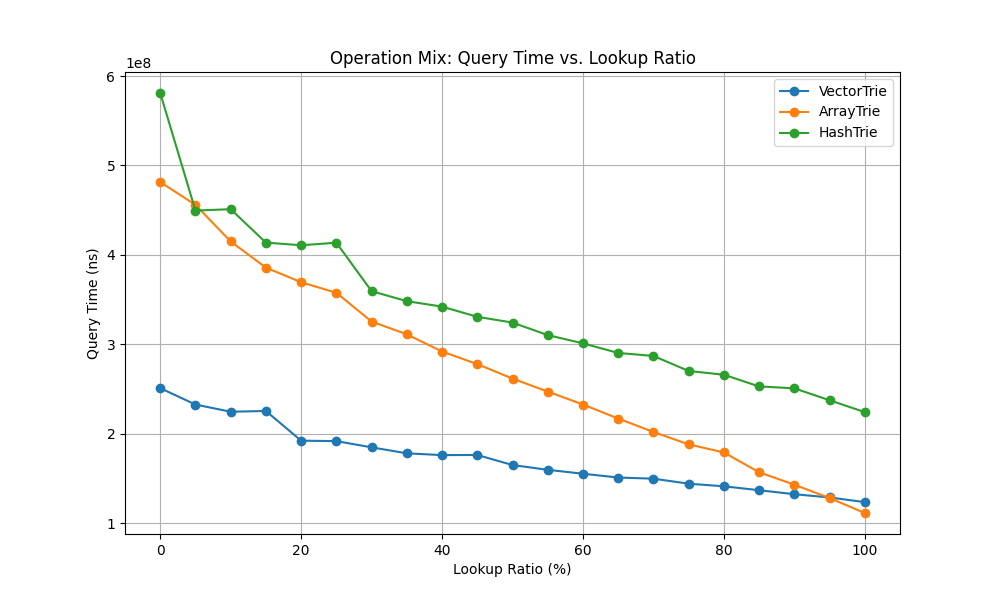
\includegraphics[width=0.8\linewidth]{plot_operation_mix/plot_operation_mix} \\
            \end{tabular}
        \end{center}
    \end{frame}

% Fill Factor Slide with images in a table (margins minimized)
    \begin{frame}{Fill Factor}
        \begin{center}
            \begin{tabular}{cc}
                \textbf{Contains}                                                                & \textbf{Insert} \\
                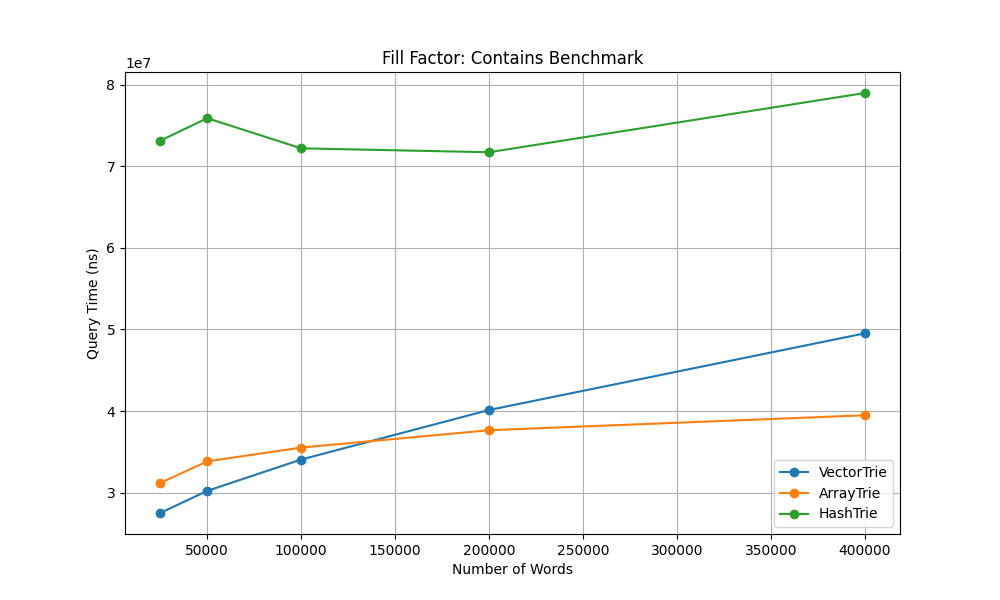
\includegraphics[width=0.45\linewidth]{plot_fill_factor/plot_fill_factor_contains} &
                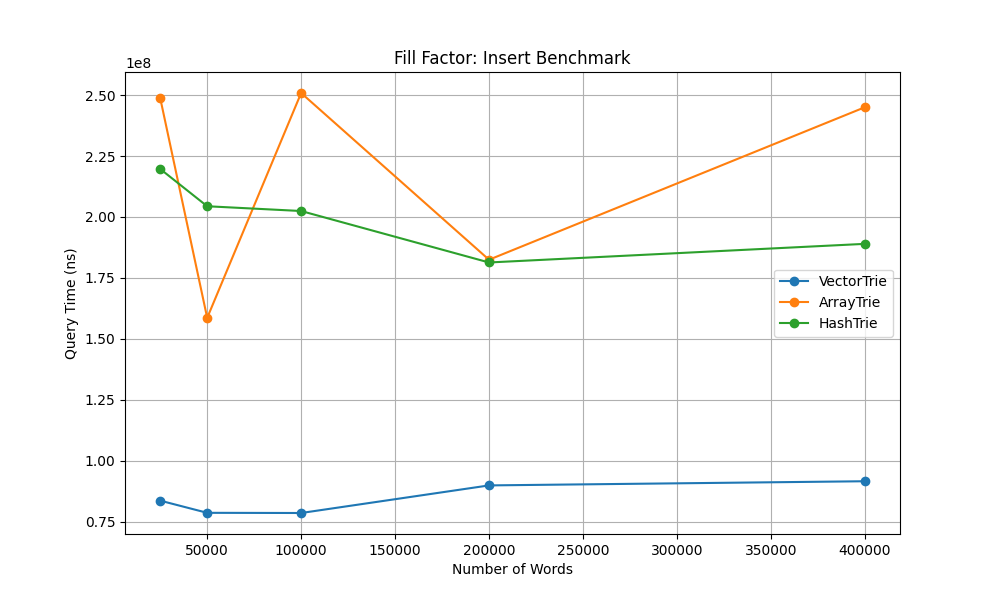
\includegraphics[width=0.45\linewidth]{plot_fill_factor/plot_fill_factor_insert} \\
                \textbf{Remove}                                                                  &                 \\
                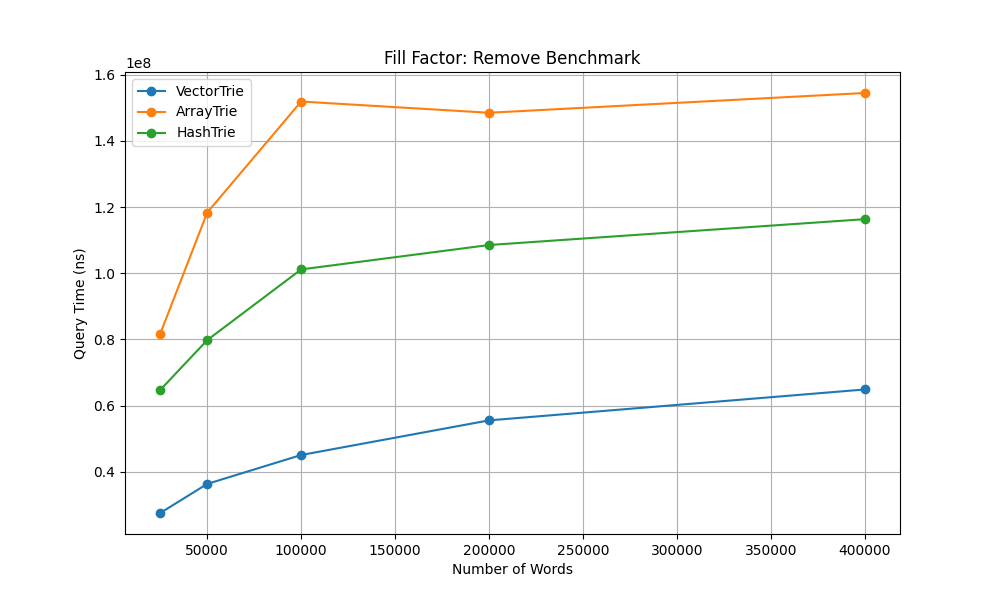
\includegraphics[width=0.45\linewidth]{plot_fill_factor/plot_fill_factor_remove}& \\
            \end{tabular}
        \end{center}
    \end{frame}

% Word Length Slides (Contains, Insert, Remove) with minimized margins

    \begin{frame}{Word Length (Contains)}
        \begin{center}
            \begin{tabular}{cc}
                \textbf{Already Inserted} & \textbf{Random String} \\
                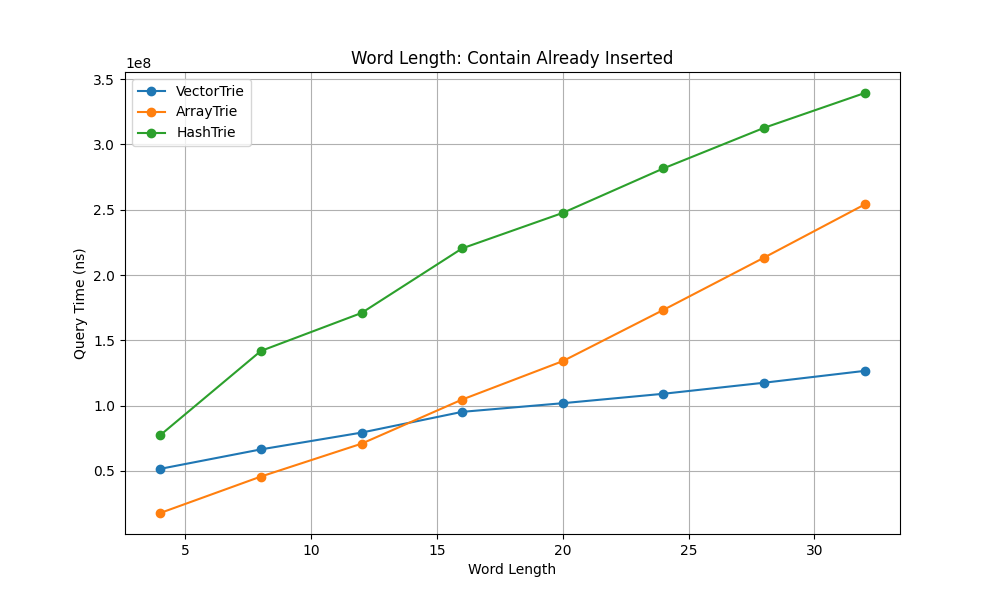
\includegraphics[width=0.48\linewidth]{plot_word_length/plot_word_length_contain_already_inserted} &
                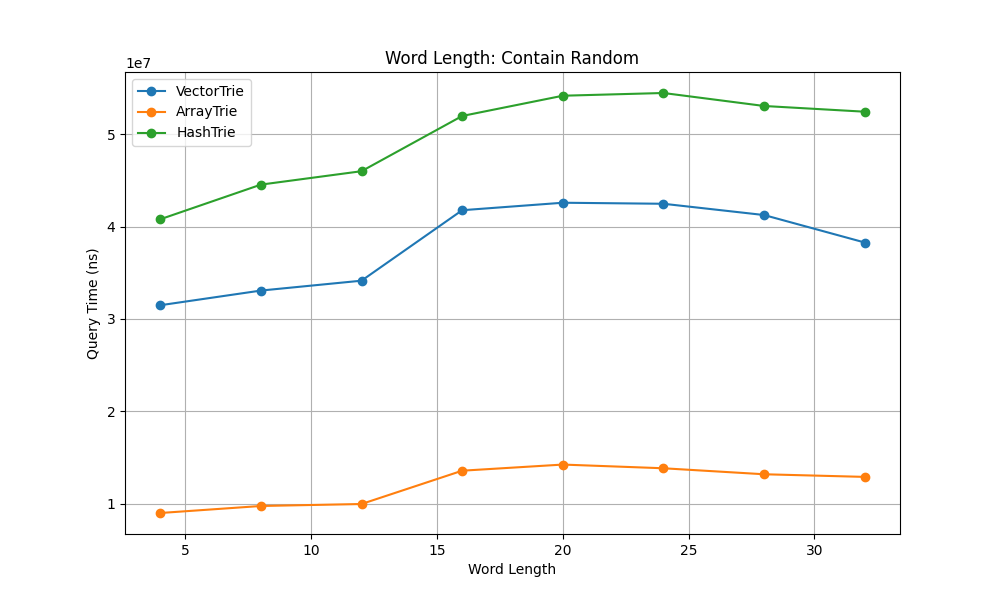
\includegraphics[width=0.48\linewidth]{plot_word_length/plot_word_length_contain_random} \\
            \end{tabular}
        \end{center}
    \end{frame}

    \begin{frame}{Word Length (Insert)}
        \begin{center}
            \begin{tabular}{cc}
                \textbf{Already Inserted} & \textbf{Random String} \\
                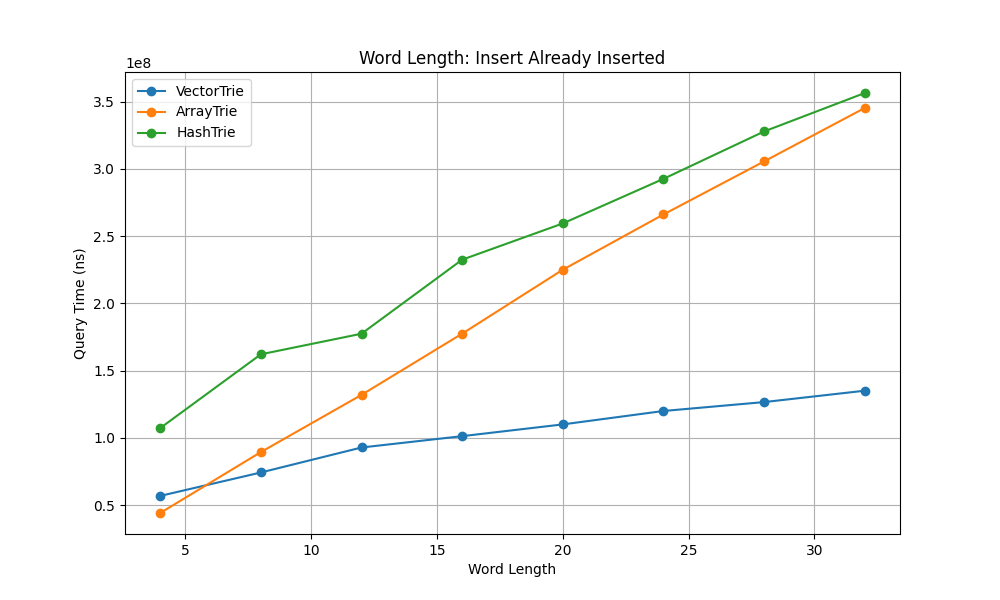
\includegraphics[width=0.48\linewidth]{plot_word_length/plot_word_length_insert_already_inserted} &
                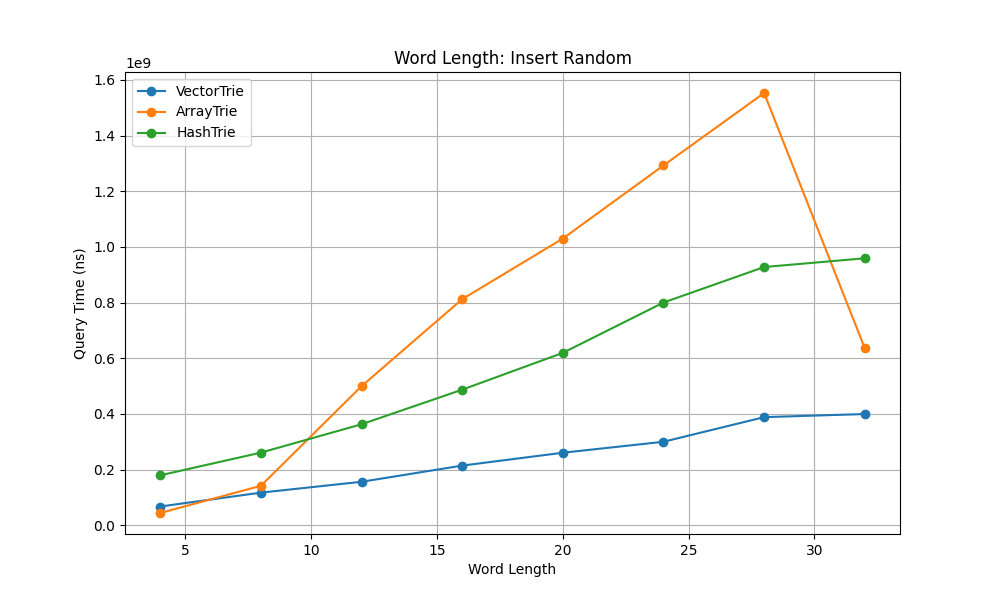
\includegraphics[width=0.48\linewidth]{plot_word_length/plot_word_length_insert_random} \\
            \end{tabular}
        \end{center}
    \end{frame}

    \begin{frame}{Word Length (Remove)}
        \begin{center}
            \begin{tabular}{cc}
                \textbf{Already Inserted} & \textbf{Random String} \\
                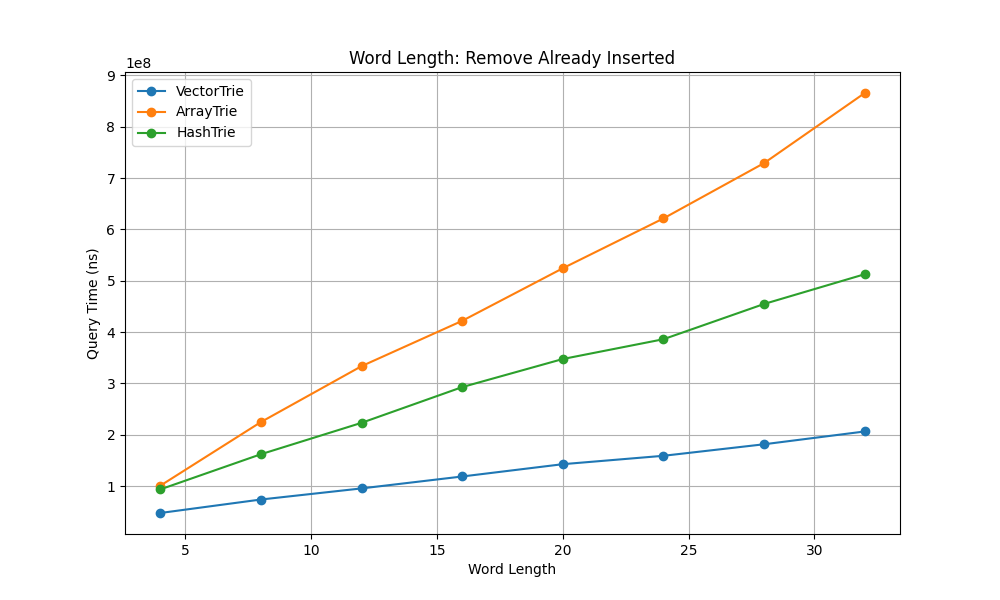
\includegraphics[width=0.48\linewidth]{plot_word_length/plot_word_length_remove_already_inserted} &
                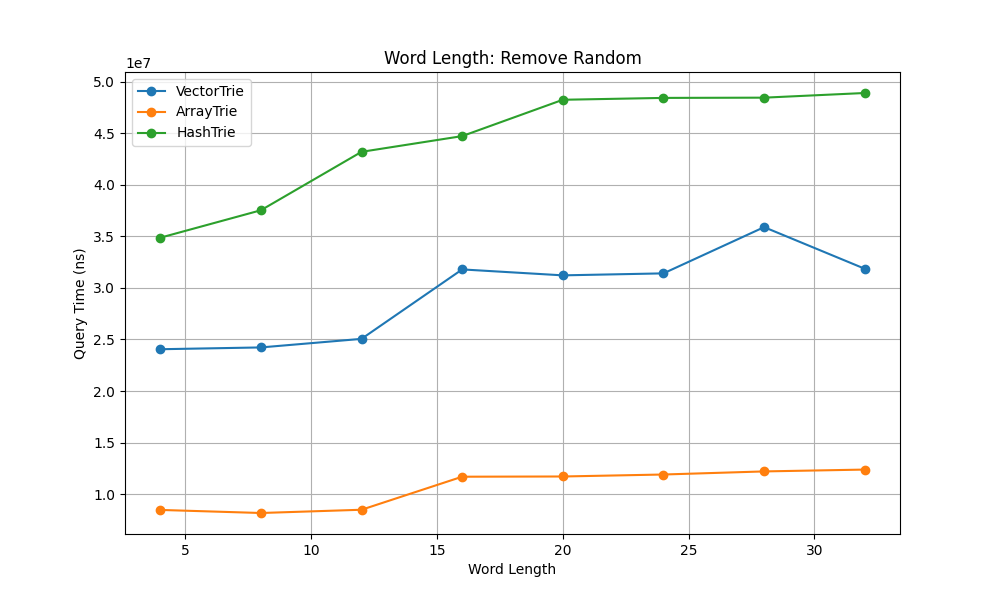
\includegraphics[width=0.48\linewidth]{plot_word_length/plot_word_length_remove_random} \\
            \end{tabular}
        \end{center}
    \end{frame}

% Construction slides: split into two

    \begin{frame}{Construction: Size}
        \begin{center}
            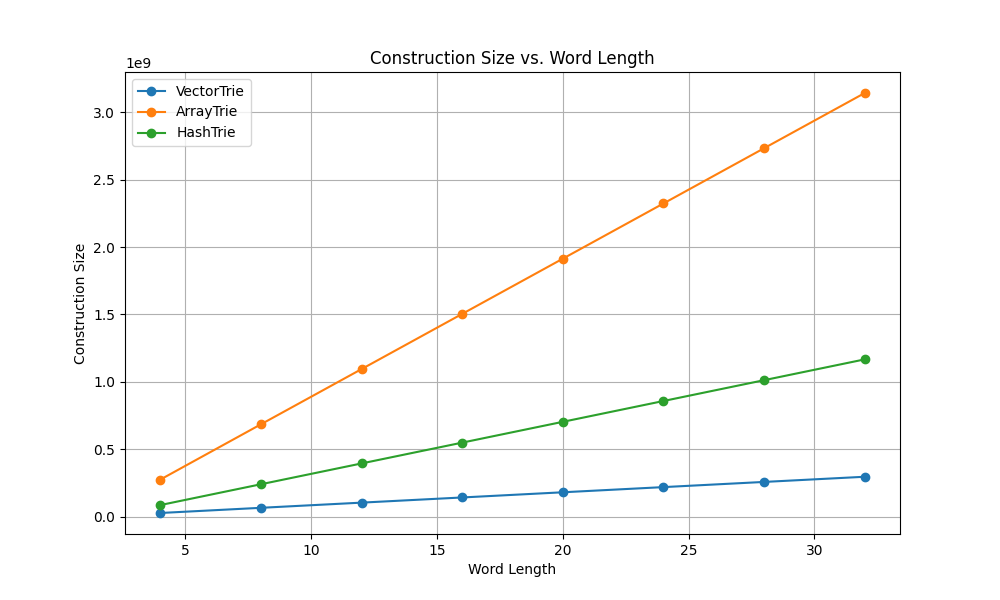
\includegraphics[width=\linewidth]{plot_word_length_construction/plot_word_length_construction_size}
        \end{center}
    \end{frame}

    \begin{frame}{Construction: Time}
        \begin{center}
            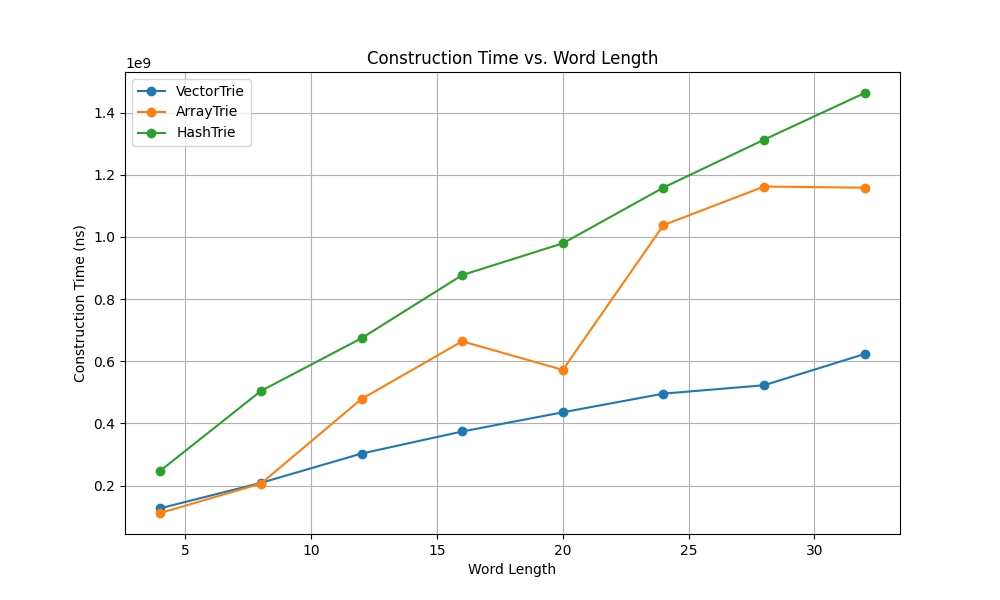
\includegraphics[width=\linewidth]{plot_word_length_construction/plot_word_length_construction_time}
        \end{center}
    \end{frame}

% Conclusion Slide
    \begin{frame}{Conclusion}
        \begin{itemize}
            \item \textbf{Hash Trie:} Not performing well.
            While using a hash map in a trie isn't always bad, this implementation is simply not smart enough.
            \item \textbf{Array Trie:} Very fast on lookup operations but suffers from significant size overhead and long construction time.
            A smarter allocation strategy (e.g., bulk allocation) might help.
            \item \textbf{Vector Trie:} The overall winner in this comparison, yielding strong performance in every scenario.
            It is the go-to solution when there is no special use-case.
        \end{itemize}
    \end{frame}

\end{document}
